\section{VL 05: Kontext Prozess I}

BPMN (Business Process Model Notation): Ansatz zur Prozessmodellierung

\begin{itemize}
  \item Prozess: Eine Folge von logischen Einzelfunktionen, zwischen denen Verbindungen bestehen. Dabei gibt es einen Auslöser der den Prozess ggf. mit Input startet.
  \item Prozessmanagement: Gestaltung, Ausführung und Beurteilung von Funktionsfolgen (Prozesse)
\end{itemize}


\subsection{Prozessmodelle}

\begin{itemize}
  \item Darstellung der Abfolgen und Verantwortlichkeiten – es lassen sich auch fehlerhafte Prozesse dokumentieren und verbessern
  \item BPMN ist ein bekannter Modellierungsansatz
\end{itemize}

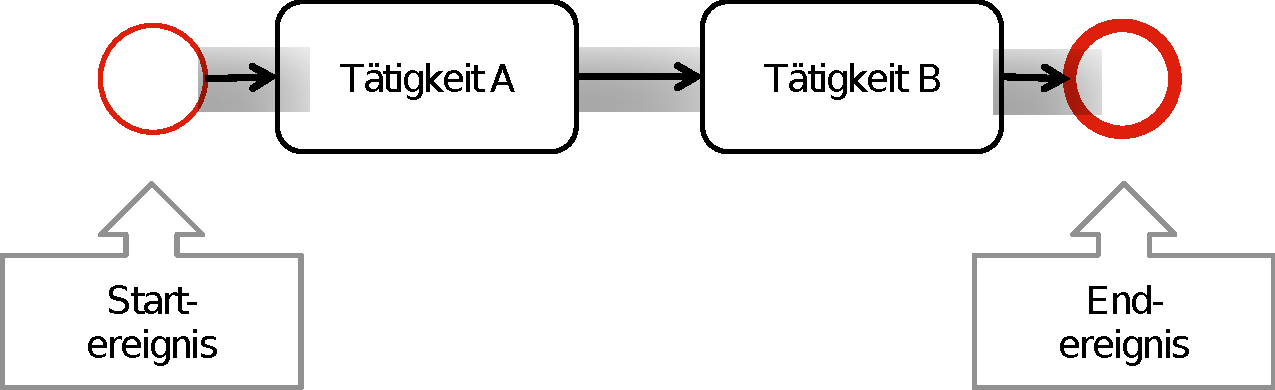
\includegraphics[width=0.7\textwidth]{5-1}

\begin{itemize}
  \item Nomen \& Verben: Was wird wie gemacht/verändert? Die Aktivitäten werden als Kästchen darstellt.
  \item Sequenzfluss: Welche Reihenfolge hat eine Tätigkeit? Die nächste Aktivität wird erst gestartet, wenn die vorherige Aktivität beendet wurde.
  \item Ereignisse: Trigger/Auslöser des Prozesses – als Kreise im Prozessdiagramm
\end{itemize}

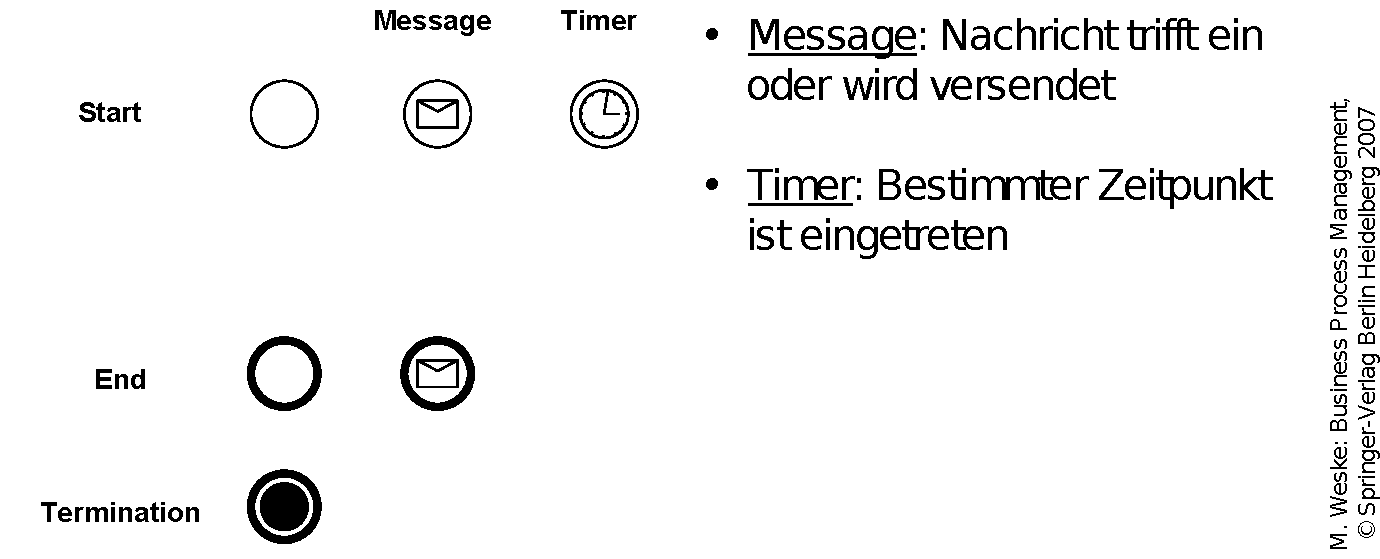
\includegraphics[width=\textwidth]{5-2}


\subsubsection{Swimmlanes und Pools}

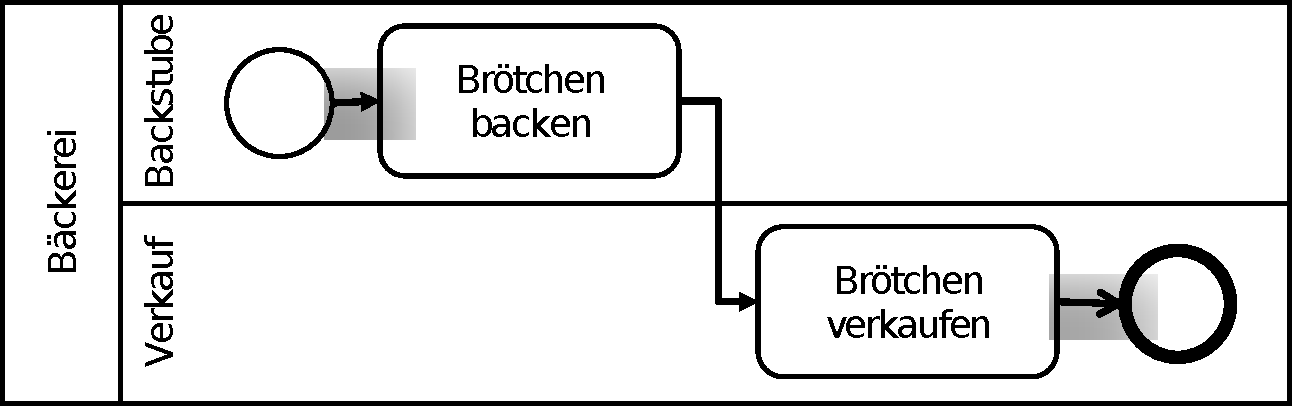
\includegraphics[width=0.7\textwidth]{5-3}

\begin{itemize}
  \item Pool ist ein Beteiligter (z.B. eine Organisation) [Bäckerei]
  \item Swimlane representiert eine Untergruppe, welche in Organisationen eingereiht werden [Verkauf, Backstube]
\end{itemize}


\subsubsection{Gateways}

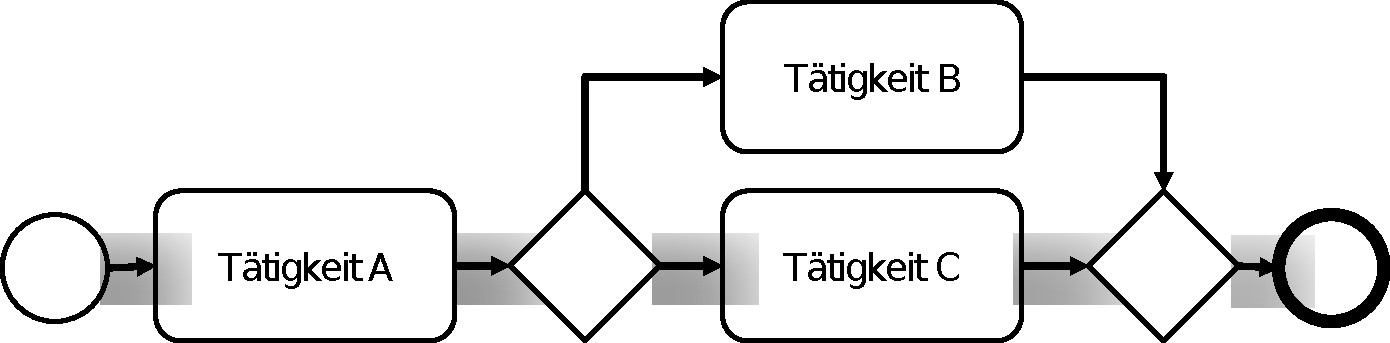
\includegraphics[width=0.7\textwidth]{5-4}

\begin{itemize}
  \item Sind eine Verzweigung der Aktivitätsfolge
  \item Regeln nach denen Prozesse ablaufen/gesteuert werden, z.B. zur Parallelisierung
  \item Exclusive Gateways: Je nach Bedingung genau eine Kante als Ausgabe. Gleiches gilt bei Zusammenführung – es muss nur eine einlaufen.
\end{itemize}

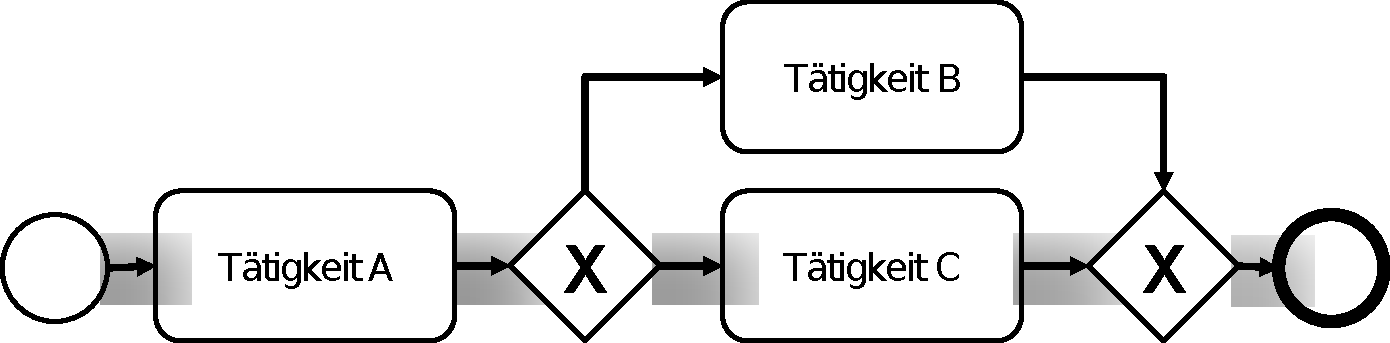
\includegraphics[width=0.7\textwidth]{5-5}

\begin{itemize}
  \item Parallele Gateways: Beide Aktivitäten werden gestartet. Beim Zusammenführen wird auch auf alle Fertigstellungen gewartet.
\end{itemize}

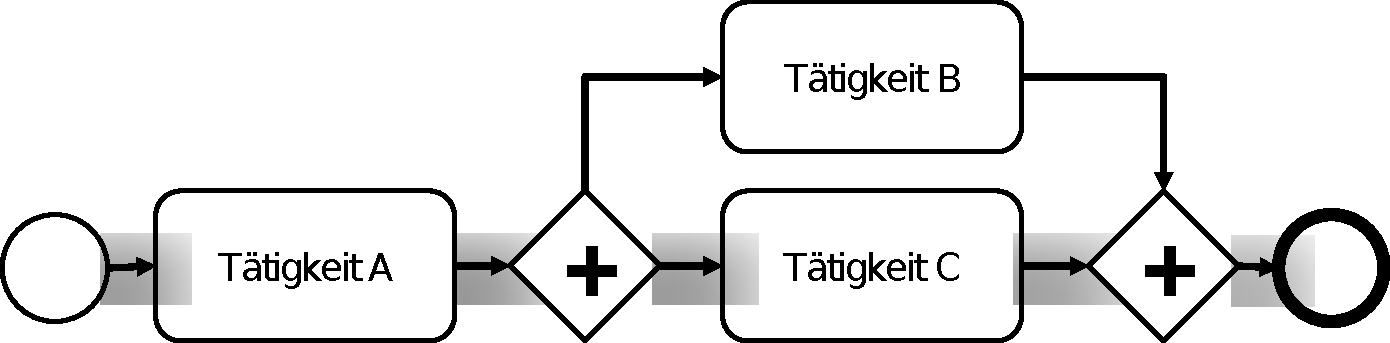
\includegraphics[width=0.7\textwidth]{5-6}